\tikzset{every picture/.style={line width=0.75pt}} %set default line width to 0.75pt        

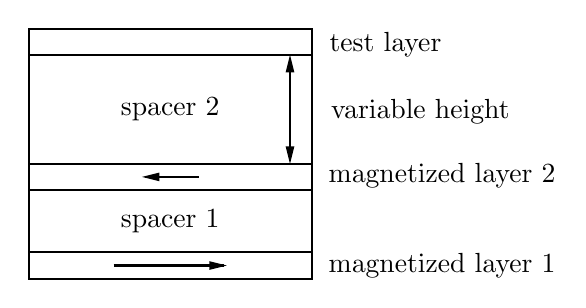
\begin{tikzpicture}[x=0.75pt,y=0.75pt,yscale=-0.7,xscale=0.7]
%uncomment if require: \path (0,300); %set diagram left start at 0, and has height of 300

%Shape: Rectangle [id:dp3897188190860059] 
\draw   (102,205.52) -- (296.83,205.52) -- (296.83,223.52) -- (102,223.52) -- cycle ;
%Shape: Rectangle [id:dp6888483467781361] 
\draw   (102,162.52) -- (296.83,162.52) -- (296.83,205.52) -- (102,205.52) -- cycle ;
%Straight Lines [id:da8737496131021489] 
\draw    (160.5,214.52) -- (236.33,214.52) ;
\draw [shift={(238.33,214.52)}, rotate = 180] [fill={rgb, 255:red, 0; green, 0; blue, 0 }  ][line width=0.08]  [draw opacity=0] (12,-3) -- (0,0) -- (12,3) -- cycle    ;
%Shape: Rectangle [id:dp7116079291498749] 
\draw   (102,144.52) -- (296.83,144.52) -- (296.83,162.52) -- (102,162.52) -- cycle ;
%Straight Lines [id:da09691248809748632] 
\draw    (181.96,153.52) -- (218.87,153.52) ;
\draw [shift={(179.96,153.52)}, rotate = 0] [fill={rgb, 255:red, 0; green, 0; blue, 0 }  ][line width=0.08]  [draw opacity=0] (12,-3) -- (0,0) -- (12,3) -- cycle    ;
%Shape: Rectangle [id:dp6421203027479565] 
\draw   (102,69.52) -- (296.83,69.52) -- (296.83,144.52) -- (102,144.52) -- cycle ;
%Shape: Rectangle [id:dp03151265514505708] 
\draw   (102,51.52) -- (296.83,51.52) -- (296.83,69.52) -- (102,69.52) -- cycle ;
%Straight Lines [id:da2218769473186446] 
\draw    (281.83,71.52) -- (281.83,142.52) ;
\draw [shift={(281.83,144.52)}, rotate = 270] [fill={rgb, 255:red, 0; green, 0; blue, 0 }  ][line width=0.08]  [draw opacity=0] (12,-3) -- (0,0) -- (12,3) -- cycle    ;
\draw [shift={(281.83,69.52)}, rotate = 90] [fill={rgb, 255:red, 0; green, 0; blue, 0 }  ][line width=0.08]  [draw opacity=0] (12,-3) -- (0,0) -- (12,3) -- cycle    ;

% Text Node
\draw (306.33,214.52) node [anchor=west] [inner sep=0.75pt]   [align=left] {magnetized layer 1};
% Text Node
\draw (199.42,184.02) node   [align=left] {spacer 1};
% Text Node
\draw (306.33,152.52) node [anchor=west] [inner sep=0.75pt]   [align=left] {magnetized layer 2};
% Text Node
\draw (199.42,107.02) node   [align=left] {spacer 2};
% Text Node
\draw (307,52) node [anchor=north west][inner sep=0.75pt]   [align=left] {test layer};
% Text Node
\draw (308,98) node [anchor=north west][inner sep=0.75pt]   [align=left] {variable height};


\end{tikzpicture}
